\section{Embedding into Sierpinski Tetrahedron}

\begin{frame}
	\frametitle{Difficulties}
	\begin{center}
	\begin{tabular}{|c|c|}
		\hline
		\textbf{Menger Sponge} & \textbf{Sierpinski Tetrahedron} \\
		\hline
		Easily understandable representation  & Difficulties caused by tetrahedrons \\
		\hline
		arc representation & ? \\
		\hline
	\end{tabular}
	\end{center}\\
	\\
	\onslide<2->
	Solution:
	\begin{itemize}
		\item Combinatorial representation of the Sierpinski Tetrahedron
		\item Pretzel knots
	\end{itemize}
	
\end{frame}

\begin{frame}
	\frametitle{Combinatorial representation of the Tetrahedron} % Changed from "Frame-titel"
	\begin{figure}[h]
		\centering
		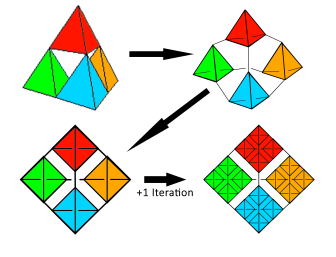
\includegraphics[width=0.5\linewidth]{images/CombRep1}
		\caption{Combinatorial representation of the Tetrahedron \cite{broden2024knotsinsidefractals}}
		\label{fig:enter-label}
	\end{figure}
\end{frame}

\begin{frame}
	\frametitle{Combinatorial representation of the Tetrahedron} % Changed from "Frame-titel"
	\begin{figure}[h]
		\centering
		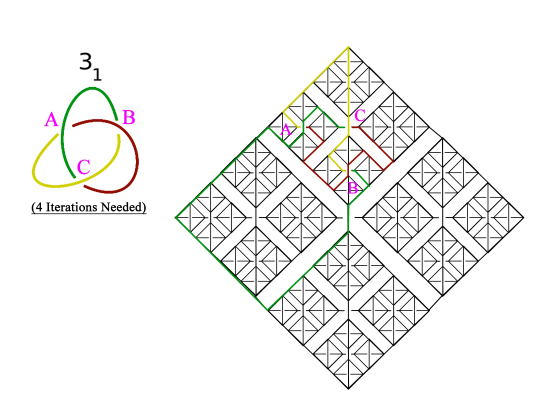
\includegraphics[width=0.5\linewidth]{images/CombRep2}
		\caption{Example $3^1$ knot \cite{broden2024knotsinsidefractals}}
		\label{fig:enter-label}
	\end{figure}
\end{frame}

\begin{frame}
	\frametitle{Combinatorial representation of the Tetrahedron} % Changed from "Frame-titel"
	\begin{figure}[h]
		\centering
		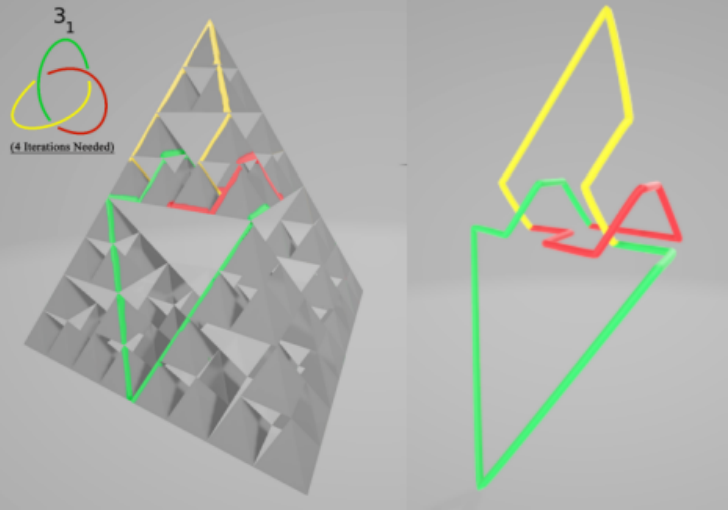
\includegraphics[width=0.5\linewidth]{images/CombRep3}
		\caption{Example $3^1$ knot \cite{broden2024knotsinsidefractals}}
		\label{fig:enter-label}
	\end{figure}
\end{frame}

\begin{frame}
	\frametitle{Sierpinski Tetrahedron} % Changed from "Frame-titel"
	\begin{theorem}
		All Pretzel Knots are inside a finite iteration of the Sierpinski Tetrahedron. \cite{broden2024knotsinsidefractals}
	\end{theorem}
\end{frame}

\begin{frame}
	\frametitle{Comparison between Fractals} % Changed from "Frame-titel"
	\begin{theorem}
		Let K be a not, then we have
		$$M(K)\leq S(K),$$
		whenever $S(K)$ is defined. \cite{broden2024knotsinsidefractals}
	\end{theorem}
	
	\onslide<2->
	\begin{proof}
		Shortly: The $i^{th}$ iteration of the Sierpinski Tetrahedron can be embedded into the Menger Sponge.
	\end{proof}
\end{frame}

\begin{frame}
	\frametitle{Comparison between Fractals} % Changed from "Frame-titel"
	\begin{figure}[!htb]
		\begin{minipage}{0.48\textwidth}
			\centering
			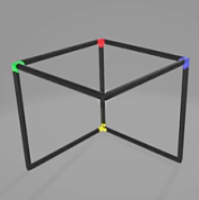
\includegraphics[width=.7\linewidth]{images/Comparison1}
			\caption{$S_0$ in $M_0$}\label{Fig:Data1}
		\end{minipage}\hfill
		\begin{minipage}{0.48\textwidth}
			\centering
			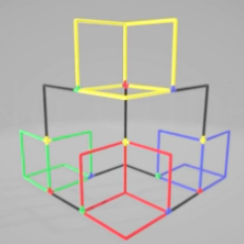
\includegraphics[width=.7\linewidth]{images/Comparison2}
			\caption{$S_1$ in $M_1$}\label{Fig:Data2}
		\end{minipage}
	\end{figure}
\end{frame}